% Options for packages loaded elsewhere
\PassOptionsToPackage{unicode}{hyperref}
\PassOptionsToPackage{hyphens}{url}
%
\documentclass[
]{article}
\usepackage{amsmath,amssymb}
\usepackage{iftex}
\ifPDFTeX
  \usepackage[T1]{fontenc}
  \usepackage[utf8]{inputenc}
  \usepackage{textcomp} % provide euro and other symbols
\else % if luatex or xetex
  \usepackage{unicode-math} % this also loads fontspec
  \defaultfontfeatures{Scale=MatchLowercase}
  \defaultfontfeatures[\rmfamily]{Ligatures=TeX,Scale=1}
\fi
\usepackage{lmodern}
\ifPDFTeX\else
  % xetex/luatex font selection
\fi
% Use upquote if available, for straight quotes in verbatim environments
\IfFileExists{upquote.sty}{\usepackage{upquote}}{}
\IfFileExists{microtype.sty}{% use microtype if available
  \usepackage[]{microtype}
  \UseMicrotypeSet[protrusion]{basicmath} % disable protrusion for tt fonts
}{}
\makeatletter
\@ifundefined{KOMAClassName}{% if non-KOMA class
  \IfFileExists{parskip.sty}{%
    \usepackage{parskip}
  }{% else
    \setlength{\parindent}{0pt}
    \setlength{\parskip}{6pt plus 2pt minus 1pt}}
}{% if KOMA class
  \KOMAoptions{parskip=half}}
\makeatother
\usepackage{xcolor}
\usepackage[margin=1in]{geometry}
\usepackage{color}
\usepackage{fancyvrb}
\newcommand{\VerbBar}{|}
\newcommand{\VERB}{\Verb[commandchars=\\\{\}]}
\DefineVerbatimEnvironment{Highlighting}{Verbatim}{commandchars=\\\{\}}
% Add ',fontsize=\small' for more characters per line
\usepackage{framed}
\definecolor{shadecolor}{RGB}{248,248,248}
\newenvironment{Shaded}{\begin{snugshade}}{\end{snugshade}}
\newcommand{\AlertTok}[1]{\textcolor[rgb]{0.94,0.16,0.16}{#1}}
\newcommand{\AnnotationTok}[1]{\textcolor[rgb]{0.56,0.35,0.01}{\textbf{\textit{#1}}}}
\newcommand{\AttributeTok}[1]{\textcolor[rgb]{0.13,0.29,0.53}{#1}}
\newcommand{\BaseNTok}[1]{\textcolor[rgb]{0.00,0.00,0.81}{#1}}
\newcommand{\BuiltInTok}[1]{#1}
\newcommand{\CharTok}[1]{\textcolor[rgb]{0.31,0.60,0.02}{#1}}
\newcommand{\CommentTok}[1]{\textcolor[rgb]{0.56,0.35,0.01}{\textit{#1}}}
\newcommand{\CommentVarTok}[1]{\textcolor[rgb]{0.56,0.35,0.01}{\textbf{\textit{#1}}}}
\newcommand{\ConstantTok}[1]{\textcolor[rgb]{0.56,0.35,0.01}{#1}}
\newcommand{\ControlFlowTok}[1]{\textcolor[rgb]{0.13,0.29,0.53}{\textbf{#1}}}
\newcommand{\DataTypeTok}[1]{\textcolor[rgb]{0.13,0.29,0.53}{#1}}
\newcommand{\DecValTok}[1]{\textcolor[rgb]{0.00,0.00,0.81}{#1}}
\newcommand{\DocumentationTok}[1]{\textcolor[rgb]{0.56,0.35,0.01}{\textbf{\textit{#1}}}}
\newcommand{\ErrorTok}[1]{\textcolor[rgb]{0.64,0.00,0.00}{\textbf{#1}}}
\newcommand{\ExtensionTok}[1]{#1}
\newcommand{\FloatTok}[1]{\textcolor[rgb]{0.00,0.00,0.81}{#1}}
\newcommand{\FunctionTok}[1]{\textcolor[rgb]{0.13,0.29,0.53}{\textbf{#1}}}
\newcommand{\ImportTok}[1]{#1}
\newcommand{\InformationTok}[1]{\textcolor[rgb]{0.56,0.35,0.01}{\textbf{\textit{#1}}}}
\newcommand{\KeywordTok}[1]{\textcolor[rgb]{0.13,0.29,0.53}{\textbf{#1}}}
\newcommand{\NormalTok}[1]{#1}
\newcommand{\OperatorTok}[1]{\textcolor[rgb]{0.81,0.36,0.00}{\textbf{#1}}}
\newcommand{\OtherTok}[1]{\textcolor[rgb]{0.56,0.35,0.01}{#1}}
\newcommand{\PreprocessorTok}[1]{\textcolor[rgb]{0.56,0.35,0.01}{\textit{#1}}}
\newcommand{\RegionMarkerTok}[1]{#1}
\newcommand{\SpecialCharTok}[1]{\textcolor[rgb]{0.81,0.36,0.00}{\textbf{#1}}}
\newcommand{\SpecialStringTok}[1]{\textcolor[rgb]{0.31,0.60,0.02}{#1}}
\newcommand{\StringTok}[1]{\textcolor[rgb]{0.31,0.60,0.02}{#1}}
\newcommand{\VariableTok}[1]{\textcolor[rgb]{0.00,0.00,0.00}{#1}}
\newcommand{\VerbatimStringTok}[1]{\textcolor[rgb]{0.31,0.60,0.02}{#1}}
\newcommand{\WarningTok}[1]{\textcolor[rgb]{0.56,0.35,0.01}{\textbf{\textit{#1}}}}
\usepackage{graphicx}
\makeatletter
\def\maxwidth{\ifdim\Gin@nat@width>\linewidth\linewidth\else\Gin@nat@width\fi}
\def\maxheight{\ifdim\Gin@nat@height>\textheight\textheight\else\Gin@nat@height\fi}
\makeatother
% Scale images if necessary, so that they will not overflow the page
% margins by default, and it is still possible to overwrite the defaults
% using explicit options in \includegraphics[width, height, ...]{}
\setkeys{Gin}{width=\maxwidth,height=\maxheight,keepaspectratio}
% Set default figure placement to htbp
\makeatletter
\def\fps@figure{htbp}
\makeatother
\setlength{\emergencystretch}{3em} % prevent overfull lines
\providecommand{\tightlist}{%
  \setlength{\itemsep}{0pt}\setlength{\parskip}{0pt}}
\setcounter{secnumdepth}{-\maxdimen} % remove section numbering
\ifLuaTeX
  \usepackage{selnolig}  % disable illegal ligatures
\fi
\IfFileExists{bookmark.sty}{\usepackage{bookmark}}{\usepackage{hyperref}}
\IfFileExists{xurl.sty}{\usepackage{xurl}}{} % add URL line breaks if available
\urlstyle{same}
\hypersetup{
  pdftitle={HW\_09},
  pdfauthor={izd3},
  hidelinks,
  pdfcreator={LaTeX via pandoc}}

\title{HW\_09}
\author{izd3}
\date{}

\begin{document}
\maketitle

Use only commands \& functions that are shown in the indicated chapter
or prior chapters.

\newpage

\hypertarget{problem-01---chapter-34-exercise-01b}{%
\subsection{Problem \#01 - Chapter 34 Exercise
\#01B}\label{problem-01---chapter-34-exercise-01b}}

\begin{Shaded}
\begin{Highlighting}[]
\CommentTok{\# Show your work here}
\FunctionTok{library}\NormalTok{(ggplot2)}
\end{Highlighting}
\end{Shaded}

\begin{verbatim}
## Warning: package 'ggplot2' was built under R version 4.2.3
\end{verbatim}

\begin{Shaded}
\begin{Highlighting}[]
\FunctionTok{library}\NormalTok{(scales)}
\NormalTok{scalesGraph000}\SpecialCharTok{+}\FunctionTok{scale\_x\_discrete}\NormalTok{(}\AttributeTok{name=}\StringTok{\textquotesingle{}Flavors\textquotesingle{}}\NormalTok{,}\AttributeTok{labels=}\FunctionTok{c}\NormalTok{(}\StringTok{\textquotesingle{}chocolate\textquotesingle{}}\NormalTok{,}\StringTok{\textquotesingle{}raspberry\textquotesingle{}}\NormalTok{,}\StringTok{\textquotesingle{}strawberry\textquotesingle{}}\NormalTok{,}
                                                        \StringTok{\textquotesingle{}vanila\textquotesingle{}}\NormalTok{))}\SpecialCharTok{+}
  \FunctionTok{scale\_fill\_manual}\NormalTok{(}\AttributeTok{values=}\FunctionTok{c}\NormalTok{(}\StringTok{\textquotesingle{}red\textquotesingle{}}\NormalTok{,}\StringTok{\textquotesingle{}white\textquotesingle{}}\NormalTok{,}\StringTok{\textquotesingle{}black\textquotesingle{}}\NormalTok{),}\AttributeTok{breaks =} \FunctionTok{c}\NormalTok{(}\StringTok{\textquotesingle{}n\textquotesingle{}}\NormalTok{,}\StringTok{\textquotesingle{}c\textquotesingle{}}\NormalTok{,}\StringTok{\textquotesingle{}s\textquotesingle{}}\NormalTok{),}
                    \AttributeTok{labels=}\FunctionTok{c}\NormalTok{(}\StringTok{\textquotesingle{}chips\textquotesingle{}}\NormalTok{,}\StringTok{\textquotesingle{}nuts\textquotesingle{}}\NormalTok{,}\StringTok{\textquotesingle{}sprinkles\textquotesingle{}}\NormalTok{),}\AttributeTok{name=}\StringTok{\textquotesingle{}Toppings\textquotesingle{}}\NormalTok{)}\SpecialCharTok{+}
  \FunctionTok{scale\_y\_continuous}\NormalTok{(}\AttributeTok{name=}\StringTok{\textquotesingle{}Frequency\textquotesingle{}}\NormalTok{,}\AttributeTok{breaks =} \ConstantTok{NULL}\NormalTok{)}
\end{Highlighting}
\end{Shaded}

\includegraphics[height=300]{3040_HW09_izd3_files/figure-latex/unnamed-chunk-1-1}

\newpage

\hypertarget{problem-02---chapter-34-exercise-02b}{%
\subsection{Problem \#02 - Chapter 34 Exercise
\#02B}\label{problem-02---chapter-34-exercise-02b}}

\begin{Shaded}
\begin{Highlighting}[]
\CommentTok{\# Show your work here}
\NormalTok{scalesGraph001}\SpecialCharTok{+}\FunctionTok{scale\_color\_manual}\NormalTok{(}\AttributeTok{breaks =} \FunctionTok{c}\NormalTok{(}\StringTok{\textquotesingle{}TRUE\textquotesingle{}}\NormalTok{,}\StringTok{\textquotesingle{}FALSE\textquotesingle{}}\NormalTok{),}\AttributeTok{values =} \FunctionTok{c}\NormalTok{(}\StringTok{\textquotesingle{}black\textquotesingle{}}\NormalTok{,}\StringTok{\textquotesingle{}red\textquotesingle{}}\NormalTok{))}
\end{Highlighting}
\end{Shaded}

\begin{verbatim}
## Warning: Using size for a discrete variable is not advised.
\end{verbatim}

\includegraphics[height=300]{3040_HW09_izd3_files/figure-latex/unnamed-chunk-2-1}

\newpage

\hypertarget{problem-03---chapter-34-exercise-04a-top-left}{%
\subsection{Problem \#03 - Chapter 34 Exercise \#04A ( top left
)}\label{problem-03---chapter-34-exercise-04a-top-left}}

\begin{Shaded}
\begin{Highlighting}[]
\CommentTok{\# Show your work here}
\NormalTok{scaled001.dat}\SpecialCharTok{|\textgreater{}}
  \FunctionTok{ggplot}\NormalTok{(}\AttributeTok{mapping =} \FunctionTok{aes}\NormalTok{(}\AttributeTok{x=}\NormalTok{weight,}\AttributeTok{y=}\NormalTok{top,}\AttributeTok{color=}\NormalTok{flav))}\SpecialCharTok{+}\FunctionTok{geom\_jitter}\NormalTok{(}\AttributeTok{shape=}\DecValTok{10}\NormalTok{)}\SpecialCharTok{+}
  \FunctionTok{scale\_color\_manual}\NormalTok{(}\AttributeTok{name=}\StringTok{\textquotesingle{}Flavors\textquotesingle{}}\NormalTok{,}\AttributeTok{breaks =} \FunctionTok{c}\NormalTok{(}\StringTok{\textquotesingle{}c\textquotesingle{}}\NormalTok{,}\StringTok{\textquotesingle{}s\textquotesingle{}}\NormalTok{,}\StringTok{\textquotesingle{}r\textquotesingle{}}\NormalTok{,}\StringTok{\textquotesingle{}v\textquotesingle{}}\NormalTok{),}
                     \AttributeTok{labels=}\FunctionTok{c}\NormalTok{(}\StringTok{\textquotesingle{}Chocolate\textquotesingle{}}\NormalTok{,}\StringTok{\textquotesingle{}Strawberry\textquotesingle{}}\NormalTok{,}\StringTok{\textquotesingle{}Raspberry\textquotesingle{}}\NormalTok{,}\StringTok{\textquotesingle{}Vanila\textquotesingle{}}\NormalTok{),}
                     \AttributeTok{values =} \FunctionTok{c}\NormalTok{(}\StringTok{\textquotesingle{}blue\textquotesingle{}}\NormalTok{,}\StringTok{\textquotesingle{}red\textquotesingle{}}\NormalTok{,}\StringTok{\textquotesingle{}black\textquotesingle{}}\NormalTok{,}\StringTok{\textquotesingle{}white\textquotesingle{}}\NormalTok{))}
\end{Highlighting}
\end{Shaded}

\includegraphics[height=300]{3040_HW09_izd3_files/figure-latex/unnamed-chunk-3-1}

\newpage

\hypertarget{problem-04---chapter-35-exercise-01d}{%
\subsection{Problem \#04 - Chapter 35 Exercise
\#01D}\label{problem-04---chapter-35-exercise-01d}}

\begin{Shaded}
\begin{Highlighting}[]
\CommentTok{\# Show your work here}
\NormalTok{scalesGraph002}\SpecialCharTok{+}\FunctionTok{scale\_y\_log10}\NormalTok{(}\AttributeTok{name=}\StringTok{"Y{-}Axis"}\NormalTok{,}\AttributeTok{breaks=}\FunctionTok{c}\NormalTok{(}\FloatTok{1.0}\NormalTok{,}\FloatTok{1.5}\NormalTok{,}\FloatTok{2.0}\NormalTok{,}\FloatTok{2.5}\NormalTok{,}\FloatTok{3.0}\NormalTok{))}
\end{Highlighting}
\end{Shaded}

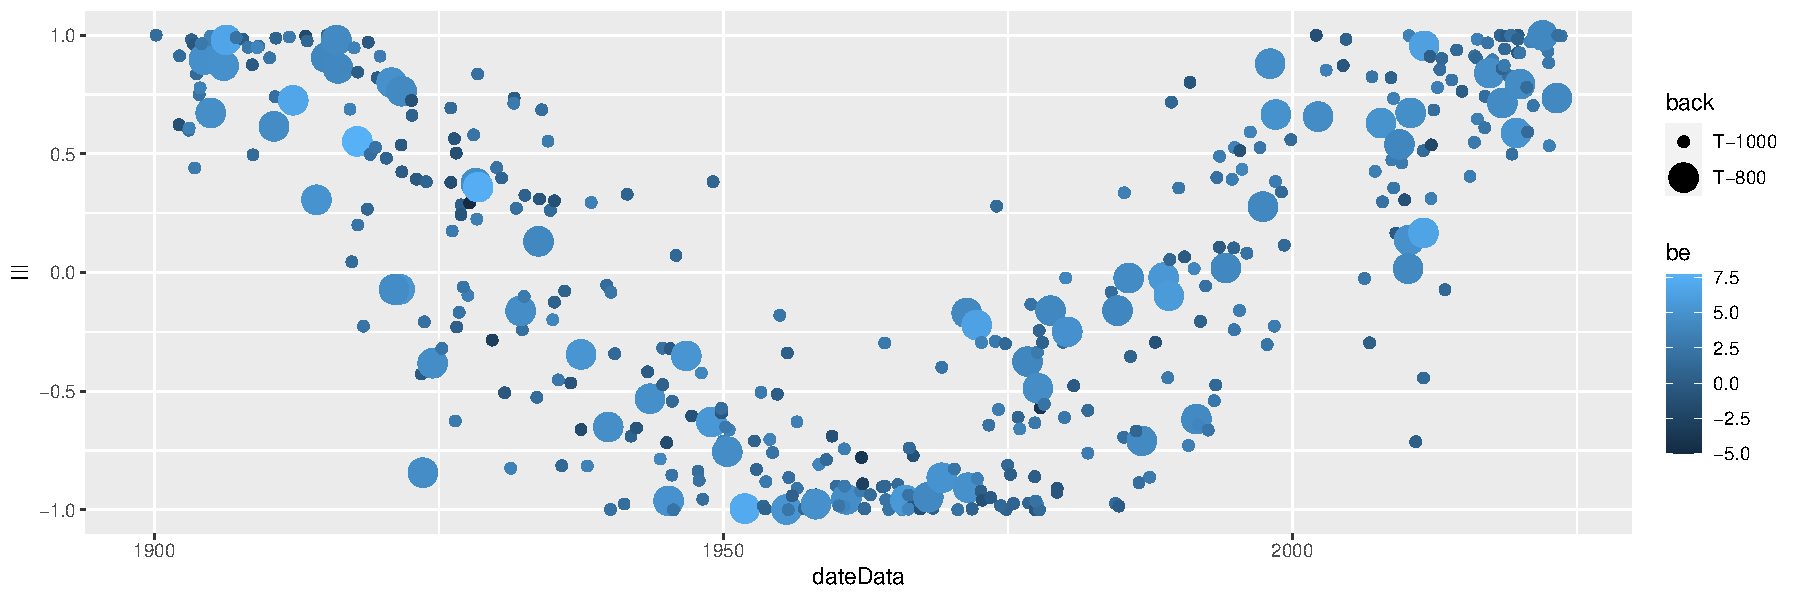
\includegraphics[height=300]{3040_HW09_izd3_files/figure-latex/unnamed-chunk-4-1}

\newpage

\hypertarget{problem-05---chapter-35-exercise-03a-red---blue}{%
\subsection{Problem \#05 - Chapter 35 Exercise \#03A (red -
blue)}\label{problem-05---chapter-35-exercise-03a-red---blue}}

\begin{Shaded}
\begin{Highlighting}[]
\CommentTok{\# Show your work here}
\NormalTok{scaled002.tib}\SpecialCharTok{|\textgreater{}}
  \FunctionTok{ggplot}\NormalTok{(}\AttributeTok{mapping =} \FunctionTok{aes}\NormalTok{(}\AttributeTok{x=}\NormalTok{var}\FloatTok{.1}\NormalTok{,}\AttributeTok{y=}\NormalTok{var}\FloatTok{.5}\NormalTok{,}\AttributeTok{color=}\NormalTok{var}\FloatTok{.3}\NormalTok{))}\SpecialCharTok{+}\FunctionTok{geom\_violin}\NormalTok{()}\SpecialCharTok{+}\FunctionTok{geom\_point}\NormalTok{()}\SpecialCharTok{+}
  \FunctionTok{scale\_x\_log10}\NormalTok{(}\AttributeTok{name=}\StringTok{\textquotesingle{}Log 10 Variable 1\textquotesingle{}}\NormalTok{,}\AttributeTok{breaks=}\FunctionTok{c}\NormalTok{(}\DecValTok{1}\NormalTok{,}\DecValTok{5}\NormalTok{,}\DecValTok{10}\NormalTok{,}\DecValTok{15}\NormalTok{))}\SpecialCharTok{+}
  \FunctionTok{scale\_color\_gradient}\NormalTok{(}\AttributeTok{name=}\StringTok{\textquotesingle{}VAR 3\textquotesingle{}}\NormalTok{,}\AttributeTok{low =} \StringTok{\textquotesingle{}red\textquotesingle{}}\NormalTok{,}\AttributeTok{high =} \StringTok{\textquotesingle{}blue\textquotesingle{}}\NormalTok{)}
\end{Highlighting}
\end{Shaded}

\begin{verbatim}
## Warning: The following aesthetics were dropped during statistical transformation: colour
## i This can happen when ggplot fails to infer the correct grouping structure in
##   the data.
## i Did you forget to specify a `group` aesthetic or to convert a numerical
##   variable into a factor?
\end{verbatim}

\includegraphics[height=300]{3040_HW09_izd3_files/figure-latex/unnamed-chunk-5-1}

\newpage

\hypertarget{problem-06---chapter-37-exercise-03b}{%
\subsection{Problem \#06 - Chapter 37 Exercise
\#03B}\label{problem-06---chapter-37-exercise-03b}}

\begin{Shaded}
\begin{Highlighting}[]
\CommentTok{\# Show your work here}
\FunctionTok{library}\NormalTok{(forcats)}
\end{Highlighting}
\end{Shaded}

\begin{verbatim}
## Warning: package 'forcats' was built under R version 4.2.3
\end{verbatim}

\begin{Shaded}
\begin{Highlighting}[]
\NormalTok{fact}\OtherTok{\textless{}{-}}\FunctionTok{factor}\NormalTok{(factorData005.fact,}\AttributeTok{levels =} \FunctionTok{c}\NormalTok{(}\StringTok{\textquotesingle{}four star\textquotesingle{}}\NormalTok{,}\StringTok{\textquotesingle{}three star\textquotesingle{}}
\NormalTok{                                           ,}\StringTok{\textquotesingle{}two star\textquotesingle{}}\NormalTok{,}\StringTok{\textquotesingle{}one star\textquotesingle{}}\NormalTok{,}\StringTok{\textquotesingle{}zero star\textquotesingle{}}\NormalTok{))}
\FunctionTok{table}\NormalTok{(fact)}
\end{Highlighting}
\end{Shaded}

\begin{verbatim}
## fact
##  four star three star   two star   one star  zero star 
##          0          0          0          7         38
\end{verbatim}

\begin{Shaded}
\begin{Highlighting}[]
\FunctionTok{unclass}\NormalTok{(fact)}
\end{Highlighting}
\end{Shaded}

\begin{verbatim}
##   [1]  4 NA  5 NA NA NA  5 NA  4  5 NA NA NA  5 NA NA  4  4 NA NA NA  5 NA NA NA
##  [26]  5  4  5  5 NA  5 NA  5  5  5 NA NA  5 NA  5  5  5  5 NA  5 NA NA  5 NA  5
##  [51] NA  5 NA NA NA NA  5 NA  5 NA NA  4 NA NA  5 NA  5  5  5  5 NA NA NA NA  5
##  [76] NA  5 NA NA  5  5  5 NA NA NA NA  5 NA NA NA  4 NA NA  5 NA NA  5  5 NA  5
## attr(,"levels")
## [1] "four star"  "three star" "two star"   "one star"   "zero star"
\end{verbatim}

\newpage

\hypertarget{problem-07---chapter-37-exercise-04b}{%
\subsection{Problem \#07 - Chapter 37 Exercise
\#04B}\label{problem-07---chapter-37-exercise-04b}}

\begin{Shaded}
\begin{Highlighting}[]
\CommentTok{\# Show your work here}
\FunctionTok{table}\NormalTok{(factorData005.fact)}
\end{Highlighting}
\end{Shaded}

\begin{verbatim}
## factorData005.fact
##  four stars    one star three stars   zero star 
##          19           7          36          38
\end{verbatim}

\begin{Shaded}
\begin{Highlighting}[]
\NormalTok{factorData005.fact}\OtherTok{\textless{}{-}}\FunctionTok{fct\_recode}\NormalTok{(factorData005.fact,}\StringTok{\textasciigrave{}}\AttributeTok{no stars}\StringTok{\textasciigrave{}}\OtherTok{=}\StringTok{"zero stars"}\NormalTok{,}\StringTok{\textasciigrave{}}\AttributeTok{one,two, or three stars}\StringTok{\textasciigrave{}}\OtherTok{=}\StringTok{\textquotesingle{}one star\textquotesingle{}}\NormalTok{,}\StringTok{\textasciigrave{}}\AttributeTok{one,two, or three stars}\StringTok{\textasciigrave{}}\OtherTok{=}\StringTok{\textquotesingle{}two stars\textquotesingle{}}\NormalTok{,}
                 \StringTok{\textasciigrave{}}\AttributeTok{one,two, or three stars}\StringTok{\textasciigrave{}}\OtherTok{=}\StringTok{\textquotesingle{}three stars\textquotesingle{}}\NormalTok{)}
\end{Highlighting}
\end{Shaded}

\begin{verbatim}
## Warning: Unknown levels in `f`: zero stars, two stars
\end{verbatim}

\begin{Shaded}
\begin{Highlighting}[]
\FunctionTok{table}\NormalTok{(factorData005.fact)}
\end{Highlighting}
\end{Shaded}

\begin{verbatim}
## factorData005.fact
##              four stars one,two, or three stars               zero star 
##                      19                      43                      38
\end{verbatim}

\newpage

\hypertarget{problem-08---chapter-33-exercise-05e}{%
\subsection{Problem \#08 - Chapter 33 Exercise
\#05E}\label{problem-08---chapter-33-exercise-05e}}

\begin{Shaded}
\begin{Highlighting}[]
\CommentTok{\# Show your work here}
\NormalTok{  test}\OtherTok{\textless{}{-}}\FunctionTok{data.frame}\NormalTok{(}\AttributeTok{factorData006.fact=}\FunctionTok{fct\_infreq}\NormalTok{(factorData006.fact),factorData004.fact}
             \OtherTok{=}\NormalTok{factorData004.fact)}
\NormalTok{test}\SpecialCharTok{$}\NormalTok{factorData004.fact}\OtherTok{=}\FunctionTok{factor}\NormalTok{(test}\SpecialCharTok{$}\NormalTok{factorData004.fact,}\AttributeTok{levels =}\NormalTok{ LETTERS[}\DecValTok{11}\SpecialCharTok{:}\DecValTok{20}\NormalTok{])}
\NormalTok{test}\SpecialCharTok{|\textgreater{}}
  \FunctionTok{ggplot}\NormalTok{(}\AttributeTok{mapping =} \FunctionTok{aes}\NormalTok{(}\AttributeTok{x=}\NormalTok{factorData006.fact,}\AttributeTok{fill=}\NormalTok{factorData004.fact))}\SpecialCharTok{+}\FunctionTok{geom\_bar}\NormalTok{()}\SpecialCharTok{+}
  \FunctionTok{scale\_fill\_manual}\NormalTok{(}\AttributeTok{breaks =}\NormalTok{ LETTERS[}\DecValTok{11}\SpecialCharTok{:}\DecValTok{20}\NormalTok{],}
                    \AttributeTok{labels=}\NormalTok{LETTERS[}\DecValTok{11}\SpecialCharTok{:}\DecValTok{20}\NormalTok{],}
                    \AttributeTok{values =} \FunctionTok{c}\NormalTok{(}\StringTok{\textquotesingle{}red\textquotesingle{}}\NormalTok{,}\StringTok{\textquotesingle{}white\textquotesingle{}}\NormalTok{,}\StringTok{\textquotesingle{}red\textquotesingle{}}\NormalTok{,}\StringTok{\textquotesingle{}white\textquotesingle{}}\NormalTok{,}\StringTok{\textquotesingle{}red\textquotesingle{}}\NormalTok{,}\StringTok{\textquotesingle{}white\textquotesingle{}}\NormalTok{,}
                               \StringTok{\textquotesingle{}red\textquotesingle{}}\NormalTok{,}\StringTok{\textquotesingle{}white\textquotesingle{}}\NormalTok{,}\StringTok{\textquotesingle{}red\textquotesingle{}}\NormalTok{,}\StringTok{\textquotesingle{}white\textquotesingle{}}\NormalTok{),}\AttributeTok{drop=}\ConstantTok{FALSE}\NormalTok{)}\SpecialCharTok{+}
  \FunctionTok{scale\_x\_discrete}\NormalTok{(}\AttributeTok{breaks=}\FunctionTok{c}\NormalTok{(}\StringTok{\textquotesingle{}reference\textquotesingle{}}\NormalTok{,}\StringTok{\textquotesingle{}gnat\textquotesingle{}}\NormalTok{,}\StringTok{\textquotesingle{}pig\textquotesingle{}}\NormalTok{),}\AttributeTok{labels=}\FunctionTok{c}\NormalTok{(}\StringTok{\textquotesingle{}REFERENCE\textquotesingle{}}\NormalTok{,}
                                                               \StringTok{\textquotesingle{}GNAT\textquotesingle{}}\NormalTok{,}
                                                               \StringTok{\textquotesingle{}PIG\textquotesingle{}}\NormalTok{))}
\end{Highlighting}
\end{Shaded}

\includegraphics[height=300]{3040_HW09_izd3_files/figure-latex/unnamed-chunk-8-1}

\end{document}
